\chapter{Class Diagram}

Di seguito viene presentato il diagramma delle classi della struttura 
\texttt{HashRBTree}, realizzato seguendo la notazione UML.

\section{Struttura Generale}

Il sistema è composto da tre elementi principali:

\begin{itemize}
    \item la struttura \texttt{KeyValue}, che rappresenta la coppia 
    chiave-valore;
    \item la classe \texttt{RBNode}, che rappresenta il nodo dell'albero;
    \item la classe \texttt{HashRBTree}, che incapsula l'intera struttura 
    dati e le operazioni su di essa.
\end{itemize}

\section{Diagramma UML}

\begin{figure}[h!]
\centering
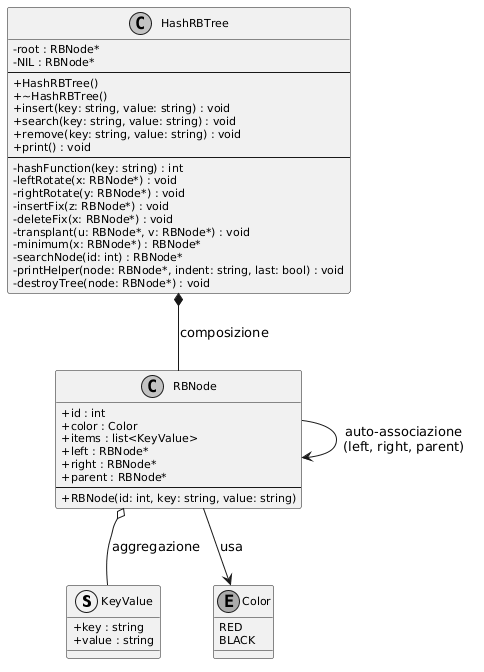
\includegraphics[width=\textwidth]{images/classdiagram.png}
\caption{Class diagram UML di HashRBTree}
\label{fig:classdiagram}
\end{figure}

\section{Relazioni tra le Classi}

\begin{itemize}
    \item \textbf{HashRBTree} ha una relazione di \textbf{composizione} con 
    \texttt{RBNode}: i nodi sono creati e distrutti esclusivamente dalla classe 
    \texttt{HashRBTree} tramite i metodi \texttt{insert} e \texttt{destroyTree}.
    \item \textbf{RBNode} ha una relazione di \textbf{aggregazione} con 
    \texttt{KeyValue}: ogni nodo contiene una \texttt{std::list<KeyValue>} 
    che può ospitare una o più coppie chiave-valore in caso di collisione.
    \item \textbf{RBNode} ha una relazione di \textbf{auto-associazione} 
    tramite i puntatori \texttt{left}, \texttt{right} e \texttt{parent}, 
    che collegano i nodi tra loro formando la struttura ad albero.
    \item Il tipo enumerato \textbf{Color} (\texttt{RED}, \texttt{BLACK}) 
    è utilizzato da \texttt{RBNode} per mantenere le proprietà cromatiche 
    del Red-Black Tree.
\end{itemize}